\documentclass[journal,10pt]{IEEEtran}
\usepackage[T1]{fontenc}
\usepackage{lmodern,cite,amsmath,amssymb,graphicx,booktabs,tabularx,array,xcolor}
\usepackage[hyphens]{url}
\usepackage[hidelinks]{hyperref}
\usepackage{balance}
\newcolumntype{Y}{>{\raggedright\arraybackslash}X}
\setlength{\emergencystretch}{2em}
\Urlmuskip=0mu plus 1mu
\title{From Clinical Reasoning to Authorized Action: A Critical Review of Agentic AI in Healthcare and a Clinical Action Assurance Framework}
\author{Anonymous research draft for author and clinical expert verification}
\begin{document}
\maketitle
\raggedbottom
\bstctlcite{IEEEcontrol}
\begin{abstract}
Healthcare AI agents increasingly retrieve evidence, operate clinical tools, and generate structured actions. Their evaluation nevertheless mixes medical knowledge, diagnostic judgment, workflow completion, and safety, obscuring what autonomy the evidence supports. This critical review develops an action-centered synthesis of 18 purposively selected empirical reports, informed by reproducible PubMed and arXiv discovery searches and primary-source checks through a literature cutoff of 10 October 2026. The sample spans collaborative medical reasoning, diagnostic dialogue, imaging tools, electronic health record sandboxes, radiotherapy planning, and administrative workflows. We distinguish a proposed action, its verified effect, and the authority to execute it. Recent benchmarks expose long-horizon, tool-protocol, and execution failures that static question answering cannot detect; retrospective patient records and actor-based evaluations remain distinct from prospective patient-care evidence. We propose Clinical Action Assurance, a reference framework combining patient binding, evidence provenance, contextual authorization, approval-bound action contracts, state verification, and monitored escalation. A synthetic reference implementation illustrates software invariants without claiming clinical validation. The resulting evaluation agenda links action-level correctness to workflow safety, human workload, equity, and patient outcomes. Reliable clinical agency requires evidence about permissible effects and their consequences.
\end{abstract}
\begin{IEEEkeywords}
Agentic artificial intelligence, clinical safety, healthcare agents, large language models, clinical evaluation.
\end{IEEEkeywords}
\section{Introduction}
\IEEEPARstart{A}{gentic} AI changes the unit of clinical evaluation. A medical language model may produce a diagnosis; an agent may decide which chart to inspect, request additional evidence, invoke an imaging tool, draft an order, and attempt to change a destination system. The correctness of the final sentence cannot establish the correctness of this entire sequence. Medical language-model and foundation-model research demonstrates substantial informational capability while also identifying limitations in clinical reasoning and human interaction \cite{singhal2023,moor2023,hager2024,goh2024}. The question for healthcare agents is what additional evidence justifies their ability to cause effects.

Agency predates language models. Classical accounts emphasize situated, goal-directed interaction \cite{wooldridge1995}. Recent architectures combine reasoning and acting, learned tool use, retrieval, and feedback memory \cite{react2023,toolformer2023,rag2020,reflexion2023}. These components can make otherwise inaccessible information available and support complex workflows. They also introduce new failure surfaces: selecting the wrong patient, reading obsolete evidence, reusing an approval after its context changes, and reporting success before a destination confirms completion. A competent planner may still issue an unauthorized action. A correctly authorized operation may still be clinically inappropriate.

Several reviews already characterize healthcare agents. A scoping review examines applications and conceptual distinctions \cite{collaco2026review}; broader surveys organize agents, architectures, evaluation, and translation challenges \cite{xu2026survey,vatsal2026taxonomy,hu2026survey}. This literature precludes a credible claim that healthcare agent review or governance is unexplored. Our contribution is a complementary analysis organized around \emph{action assurance}: a proposed operation, an observed effect, and the institutional authority that permits that effect. Table~\ref{tab:position} makes the intended distinction explicit without assuming that prior reviews omit safety or tool use.

We ask three questions. First, what kind of agency and destination effect do empirical reports actually evaluate? Second, which failure mechanisms emerge between a plausible proposal and a verified, permissible effect? Third, how should software controls and clinical evaluation be connected before agents receive bounded operational authority? We address these questions through a purposive evidence map and propose Clinical Action Assurance (CAA), a reference framework with a synthetic implementation. CAA is a synthesis and operationalization of existing principles, not a certification scheme or a proof that an agent is safe. The Outstanding Questions box identifies priorities for clinical translation.

\begin{table}[t]
\caption{Positioning relative to existing review literature}
\label{tab:position}\centering\footnotesize
\begin{tabularx}{\columnwidth}{@{}p{.23\columnwidth}Y@{}}\toprule
Source & Complementary emphasis \\ \midrule
Collaco et al. \cite{collaco2026review} & Scoping of applications and agentic conceptual features.\\
Xu et al. \cite{xu2026survey} & Broad survey of AI agents in healthcare.\\
Vatsal et al. \cite{vatsal2026taxonomy} & Taxonomic treatment of healthcare agent capabilities.\\
Abdollahi et al. \cite{hu2026survey} & Biomedical engineering survey of agents and translation.\\
Present review & Action/effect/authority distinctions; traceable evidence limits; approval and destination-state obligations.\\ \bottomrule
\end{tabularx}
\end{table}

\section{Review Design and Methods}
\subsection{Scope and analytical approach}
This is a critical integrative review with purposive selection, not a systematic review, scoping review, or meta-analysis. The modern empirical scope is January 2022 to 10 October 2026; earlier sources provide conceptual, uncertainty, and reporting context. The protocol was developed during scoping and was not preregistered. We use transparency elements consistent with sound narrative review practice \cite{sanra2019}, but do not claim PRISMA or PRISMA-ScR compliance \cite{prisma2020,prismascr2018}. The accompanying supplement specifies queries, selection rationale, extraction fields, access restrictions, and unresolved author checks.

We operationally include LLM-based healthcare systems that iterate over observations and decisions, use external tools, orchestrate components, or generate structured action proposals. Medical question answering and diagnostic dialogue are included selectively as boundary comparators: they help identify what an execution claim would require beyond a high-quality answer. Unrelated robotic control, marketing-only accounts, and unverified deployment descriptions do not provide empirical anchors for this analysis.

\subsection{Discovery and purposive selection}
Reproducible PubMed and arXiv queries combine agent terminology with clinical and healthcare terms. PubMed publication dates and arXiv submitted dates have different meanings; the scripts preserve those database-specific restrictions. Targeted retrieval from primary journal, conference, and preprint sources supplements database discovery. The original temporary exports were unavailable after an interrupted upload; the accompanying inventory is a newly retrieved snapshot, with its own timestamps. Historical counts are not presented as recovered data.

The metadata inventory is an \emph{unassessed discovery inventory}. It is not a screening flow or a denominator for publication prevalence. Identifier-level duplicate removal does not resolve article/preprint versions. Eighteen empirical reports are selected to cover diagnostic dialogue, collaborative reasoning, imaging tools, EHR tasks, management, radiotherapy planning, and administration. Eight are journal reports, four are conference reports, and six are preprints under the cited publication versions. Two are boundary comparators. These counts describe this selected map, not the literature as a whole. The absence of a particular deployment design in the map cannot establish that it does not exist elsewhere.

\subsection{Extraction and verification}
For each report we record a persistent identifier, publication status, task/sample unit, environment, tool or action type, observable effect, endpoint, reported quantitative anchor, source locator, and interpretation limit. Primary-source access is logged separately from metadata resolution. GPTPlan is extracted from its abstract only \cite{gptplan2025}; claims about its detailed implementation or patient outcomes are therefore not made. Cited versions and institutional sources take precedence over secondary news summaries.

Extraction and synthesis were AI-assisted. No independent dual screening, human consensus adjudication, agreement statistic, or formal risk-of-bias score is reported. The claim register marks independent author verification as pending. Clinical and methodological reviewers should confirm every quantitative anchor and its denominator before submission. We avoid pooling because task definitions, model configurations, tool budgets, evidence access, and scoring differ. The framework and illustrative software are original analytical outputs; they are not additional clinical efficacy evidence.

\section{From Informational Agency to Operational Authority}
\subsection{Capability and authority are separate axes}
We define clinical agency as the capacity to choose and perform steps toward a healthcare task while interacting with an environment. Operational authority is permission, grounded in institutional context, to produce specified effects. A system can have extensive reasoning and tool capability but no permission to write clinical state. Conversely, a narrow automation can have permission to perform one operation without general reasoning. Figure~\ref{fig:agency} separates these dimensions.

A deployment description should identify what the agent can observe, propose, and commit; what a human must approve; and how completion is verified. ``Autonomous'' without these boundaries is insufficient. Local hosting governs infrastructure and data access, but cannot establish whether a clinical action is appropriate. Multi-agent debate can alter the reasoning process, but does not create institutional permission or independent clinical judgment.

\begin{figure}[t]\centering
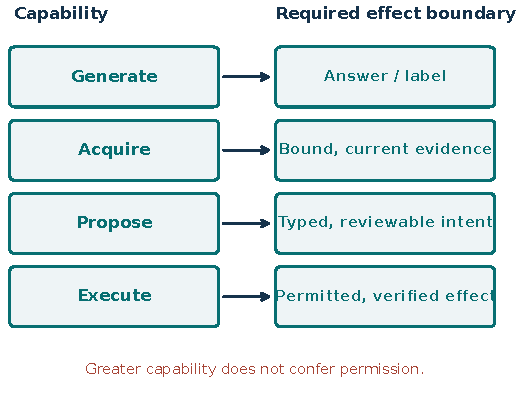
\includegraphics[width=\columnwidth]{figures/fig1_agency_authority.pdf}
\caption{Agency and authority are distinct. Each increased capability requires an explicit effect boundary and corresponding evidence; position does not imply clinical readiness.}\label{fig:agency}
\end{figure}

\begin{table}[t]\caption{Observable action classes and required distinctions}\label{tab:actions}\centering\footnotesize
\begin{tabularx}{\columnwidth}{@{}p{.23\columnwidth}YY@{}}\toprule
Class & Observable object & Essential distinction \\ \midrule
Informational answer & Text or label & Answer accuracy versus clinical effect.\\
Evidence acquisition & Retrieved observation & Availability versus freshness and patient binding.\\
Structured proposal & Typed operation & Plausible intent versus authorized commitment.\\
Sandbox commitment & Verified test-state change & Execution success versus real care.\\
Live bounded commitment & Destination receipt and state & Authorization versus clinical appropriateness.\\
Longitudinal delegation & Effects over time & Single action versus monitoring, omission, and recovery.\\ \bottomrule
\end{tabularx}\end{table}

\subsection{A trajectory is more than its final output}
For a task episode, let
\begin{equation}
\tau=\{(o_t,a_t,r_t,s_{t+1})\}_{t=1}^{T},
\end{equation}
where $o_t$ is an observation, $a_t$ a proposed or submitted action, $r_t$ a tool or destination receipt, and $s_{t+1}$ the subsequent state. The agent generally sees only part of the true clinical and technical state. A successful tool response may mean that a request was accepted, not that the intended effect occurred. A generated summary can claim completion despite an empty or incorrect destination result. Evaluators must therefore specify the state predicate that counts as success, how it is observed, and when that observation expires.

A write to a sandbox chart and a write to a live clinical record may use the same interface, yet have different authority and consequences. Table~\ref{tab:actions} distinguishes them. This taxonomy also separates research artifacts, such as executable analysis code, from clinical operations such as ordering a test. The former can be verified against software tasks without implying the latter are suitable for unsupervised use.

\subsection{Architecture does not determine evidence strength}
Single-agent loops, planner--executor arrangements, specialist panels, and multi-agent critics represent useful design options. Evidence should attach to a fully specified configuration: model/version, prompts, memory, retrieval corpus, tools, permissions, stopping rules, and budgets. Feedback memory may improve performance on a repeated task distribution while also changing the system being evaluated. Retrieval can ground answers in supplied material while exposing the planner to misleading or adversarial instructions. More components can add opportunities for cross-checking and also create correlated failure, inconsistent state, and communication overhead. The appropriate comparator is a matched workflow, not an architectural label.

\section{What the Selected Evidence Supports}
Figure~\ref{fig:evidence} maps the selected reports by publication status, environment, action, and endpoint. It is categorical: neither rows nor colors define a performance ranking. The central pattern is a progression from answers and dialogue toward verifiable benchmark effects, with persistent separation between simulation and live patient care.

\begin{figure*}[t]\centering
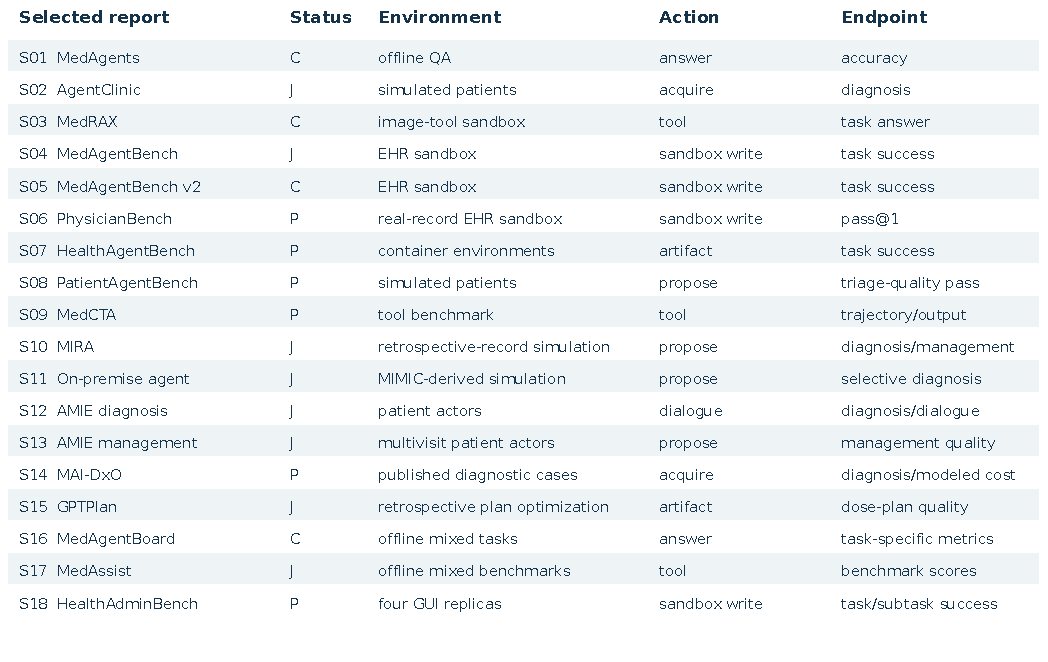
\includegraphics[width=\textwidth]{figures/fig2_evidence_map.pdf}
\caption{Purposive evidence map of 18 empirical reports. J: journal; C: conference; P: preprint. Environments and endpoints are recorded under the cited versions. These categories do not measure prevalence, quality scores, or clinical readiness.}\label{fig:evidence}
\end{figure*}

\subsection{Reasoning and diagnostic interaction}
MedAgents studies collaborative medical reasoning on question-answering tasks \cite{medagents2024}. It is useful as a boundary comparator because an improved answer does not verify a clinical action. AgentClinic introduces interactive simulated patient evaluation \cite{agentclinic2026}, moving the assessment toward information acquisition. MedRAX combines medical imaging tools with an agent workflow \cite{medrax2025}; success remains attached to benchmark queries rather than prospective radiology decisions.

AMIE evaluates diagnostic consultation with patient actors \cite{amie2025}. Its management extension investigates multivisit, guideline-grounded interaction \cite{amiemanagement2026}. These designs provide richer assessments of dialogue and recommendations than static examination questions. Actors, however, are not patients receiving autonomous treatment. Neither a conversational recommendation nor an actor-based outcome verifies that a medication order was admissible, committed correctly, and followed safely. MAI-DxO evaluates sequential information gathering on 304 published diagnostic cases and models testing cost \cite{maid2025}. Modeled test cost must not be interpreted as measured expenditure or effectiveness in routine care.

\subsection{Execution-grounded EHR and tool tasks}
MedAgentBench evaluates 300 tasks over 100 patient profiles in an EHR sandbox \cite{medagentbench2025}. Its second version reports different conditions on original and new tasks \cite{medagentbenchv2}. The memory-related results and newly constructed tasks require separate interpretation; combining them would obscure both feedback exposure and distribution shift.

PhysicianBench uses real-record EHR tasks with script-verified checkpoints \cite{physicianbench2026}. Its 100 long-horizon tasks involve 670 checkpoints and an average of 27 calls. The best reported pass@1 is 46\%. This is stronger evidence of execution difficulty than a static QA score, but still evidence from a benchmark environment. The title's ``real-world'' wording describes grounding and workflow realism; it should not be converted into a prospective deployment claim.

HealthAgentBench spans 54 tasks in seven categories with distinct environments and executable artifacts \cite{healthagentbench2026}. PatientAgentBench studies simulated patient interaction and triage \cite{patientagentbench2026}. MedCTA evaluates tool-use trajectories as well as outputs \cite{medcta2026}. Together these reports make task completion, intermediate decisions, and evaluation definitions more visible. Their scores remain conditional on supplied environments and adjudication methods.

\begin{table*}[t]\caption{Selected quantitative anchors: preserve endpoint and context}\label{tab:anchors}\centering\footnotesize
\begin{tabularx}{\textwidth}{@{}p{.15\textwidth}p{.35\textwidth}Y@{}}\toprule
Report & Reported anchor & Interpretation boundary \\ \midrule
MedAgentBench v2 \cite{medagentbenchv2} & Original tasks: 91\% without memory, 98\% with feedback memory; new tasks: 266/300 (88.67\%). & Distinct sets/configurations; not a pooled estimate.\\
PhysicianBench \cite{physicianbench2026} & 100 tasks, 670 checkpoints, average 27 calls; best 46\% pass@1. & Real-record sandbox execution; not live clinical utility.\\
HealthAgentBench \cite{healthagentbench2026} & 54 tasks, seven categories; best approximately 42\% task success. & Heterogeneous artifact tasks; no cross-benchmark ranking.\\
PatientAgentBench \cite{patientagentbench2026} & 1,200 scenarios, ten models; triage-quality pass rates 32--88\%. & Model/scenario-dependent triage; no verified downstream effect.\\
MedCTA \cite{medcta2026} & 107 tasks and five tools. & Dataset scale, not clinical efficacy or harm rate.\\
MIRA \cite{mira2026} & More than 500 cases, 11 tools, over 85,000 possible actions. & Retrospective simulation and physician comparisons.\\
On-premise agent \cite{onprem2026} & Consistency threshold 0.90: 49.4\% retained, 98.9\% diagnostic accuracy. & Selective diagnostic endpoint; not unsafe committed-action risk.\\
GPTPlan \cite{gptplan2025} & 12 lung IMRT and five cervical VMAT cases. & Abstract-only plan evaluation; no treatment-delivery claim.\\
HealthAdminBench \cite{healthadmin2026} & 135 tasks, 1,698 points; best task 36.3\%; highest subtask 82.8\%. & Different agent configurations achieve the two maxima.\\ \bottomrule
\end{tabularx}\end{table*}

\subsection{Clinical management, planning, and administration}
MIRA integrates diagnostic and management options in retrospective clinical simulations \cite{mira2026}. Its broad tool/action space and physician comparisons make it relevant to action-centered evaluation, but do not establish prospective autonomous patient care. An on-premise system examines operational governance and diagnostic reliability using MIMIC-derived environments \cite{onprem2026,mimiciv2023}. Selective retention of more consistent diagnoses is an important uncertainty result. It does not demonstrate the same risk for committed orders, omission, or downstream outcomes.

GPTPlan concerns radiotherapy plan optimization \cite{gptplan2025}. A generated treatment plan is an artifact that requires further verification and authorization before delivery. Because access here is abstract-only, no detailed claim about its control architecture is used. MedAgentBoard compares approaches across several offline medical tasks \cite{medagentboard2025}; MedAssist evaluates a general tool-oriented agent configuration \cite{medassist2026}. These mixed-task studies caution against treating multi-agent design as an inherent benefit. Additional medical-agent evaluation work likewise motivates explicit task and interface definitions \cite{medicalagentsbench2026}.

HealthAdminBench provides four GUI replicas for EHR, payer, and document workflows \cite{healthadmin2026}. The contrast between task and subtask rates is especially instructive: the reported best end-to-end task success and highest subtask success come from different configurations. Administrative effects can influence care access, eligibility, and delay. Their consequences require evaluation even when the agent never issues a clinical order.

\subsection{Synthesis across heterogeneous endpoints}
Table~\ref{tab:anchors} preserves units and limitations. Three deductions follow from the selected evidence. First, interaction and execution create additional testable failure modes beyond knowledge recall. Second, realistic records or interfaces improve fidelity without removing the distinction between sandbox and clinical deployment. Third, benchmark completion is a necessary capability measure for some workflows but is not sufficient evidence of patient benefit or admissible autonomy. None of the selected reports, under the extracted evaluation designs, establishes prospective autonomous live patient-care effectiveness. This statement is limited to the selected map and is not an assertion about all systems worldwide.

\section{Failure Mechanisms Between Proposal and Effect}
\subsection{Identity, evidence, and temporal context}
An agent can reason coherently about the wrong record. A patient identifier in the prompt is insufficient if tool sessions, active encounters, or destination adapters refer to different subjects. Binding must be enforced at the data and action boundary, with explicit conflict handling. Likewise, evidence can be true but no longer relevant: medications change, new results appear, and pending orders are completed elsewhere. A contract must identify the resource versions and validity interval on which its proposal depends.

This creates a time-of-check/time-of-use problem. A clinician may approve a proposal based on one state; execution may occur after that state changes. Rechecking just before a write reduces exposure but does not by itself prevent a concurrent change. Where supported, the destination must enforce atomic version preconditions or equivalent transactional controls. Where unsupported, the residual risk and human workflow must be specified rather than hidden behind a generic ``verified'' label.

\subsection{Adversarial content and correlated reasoning}
Agents ingest chart notes, retrieved documents, and tool outputs that may contain instructions. A prompt-injection study on medical advice demonstrates that adversarial content can distort outputs \cite{leeinjection2025}. Its attack results should not be interpreted as a production incidence rate. Medical prompt-injection benchmarks and firewall research extend this concern \cite{mpib2026,qfire2026}; detection remains configuration- and threat-dependent. Untrusted content must never obtain authority to expand tool scope or approve an action. Technical permission should come from a trusted policy boundary.

A critic or second agent does not automatically provide an independent safety check. Shared models, training, retrieval, and prompts may create correlated errors. A majority vote can be confidently wrong, and an approving explanation can lack the information needed to assess a destination effect. The appropriate tests include adversarial retrieval, contradictory records, inaccessible data, and heterogeneous execution states, not only agreement among language-model outputs.

\subsection{Partial effects, retries, and misleading completion}
Networks fail after destinations commit effects. A timeout can therefore mean either no effect or an unknown effect. Blind retry can duplicate an order or task. Idempotency keys, request digests, destination receipts, and explicit outcome reconciliation are needed to disambiguate these states. ``Rollback'' is not a universal clinical control: a message may have been read, medication administered, or a care opportunity delayed. Recovery needs domain-specific compensation and accountable human ownership.

\begin{table*}[t]\caption{Failure triggers, test obligations, and residual limits}\label{tab:failure}\centering\footnotesize
\begin{tabularx}{\textwidth}{@{}p{.16\textwidth}p{.30\textwidth}Y@{}}\toprule
Failure trigger & Test obligation & Candidate control and its limit \\ \midrule
Wrong patient/encounter & Swap trusted subject or active adapter binding. & Bind context and contract; identity systems can still be erroneous.\\
Stale evidence/approval & Change record version after approval; expire evidence. & Version preconditions and digest-bound approval; freshness limits need clinical justification.\\
Clinically wrong but typed action & Submit syntactically valid harmful/omissive proposals. & Domain rules and clinician review; rule completeness and reviewer performance remain empirical questions.\\
Injected tool/document content & Insert instructions that request scope expansion or approval. & Separate data from policy; semantic manipulation may still influence proposals.\\
Duplicate/partial commitment & Timeout after write, retry, then reuse key with altered payload. & Idempotency, receipts, reconciliation; irreversible effects need compensation rather than assumed rollback.\\
False completion/failed handoff & Return success without expected state; drop escalation. & Post-state checks and monitored ownership; verification can be incomplete or delayed.\\ \bottomrule
\end{tabularx}\end{table*}

\subsection{Long horizons and omissions}
Let $B_t$ denote an acceptable step, defined for a particular task. The chain rule gives
\begin{equation}
\Pr\!\left(\bigcap_{t=1}^{T}B_t\right)=\prod_{t=1}^{T}\Pr(B_t\mid B_1,\ldots,B_{t-1}).
\end{equation}
Only under a deliberately simplified constant, independent-step model does this become $p^T$. Figure~\ref{fig:horizon} illustrates that mathematical sensitivity, not a clinical error estimate. Actual failures can be dependent and can be detected or recovered; different steps have different consequences. No published benchmark rate is substituted for $p$.

Action correctness also misses harmful inaction. A system can complete every attempted operation while failing to notice a critical task, deferring beyond its deadline, or escalating without effective follow-through. Safety analysis must include omissions and availability of the human fallback. Table~\ref{tab:failure} connects these mechanisms to falsifiable control obligations.

\begin{figure}[t]\centering
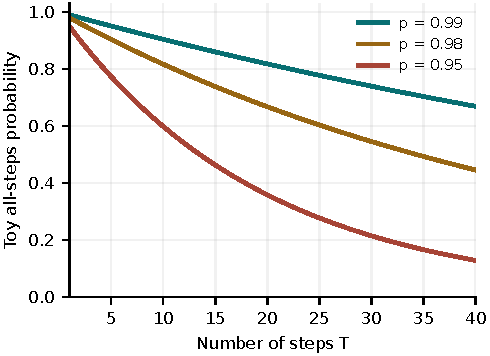
\includegraphics[width=\columnwidth]{figures/fig4_horizon_toy.pdf}
\caption{Illustrative $p^T$ under constant independent step acceptability. Curves are mathematical examples, not clinical data, estimated harm probabilities, or benchmark projections.}\label{fig:horizon}
\end{figure}

\section{Clinical Action Assurance Framework}
\subsection{Purpose and trust boundary}
CAA is a proposed reference framework for connecting clinical evidence, institutional authority, bounded execution, and verified effects. It draws on lifecycle governance and risk-management principles \cite{who2024,nist2023,nist2024,governingagents2023}, as well as interoperable authorization and provenance mechanisms \cite{smart2024,fhir2019}. These sources do not certify an agent's clinical safety. CAA makes explicit the software and clinical assumptions needed to operationalize them.

Figure~\ref{fig:caa} places policy and identity outside the planner. An institutionally trusted context supplies the initiating principal, purpose, patient, encounter, policy version, permitted operations, and required reviewer. The planner can propose typed actions based on an evidence workspace; it cannot mint its own permissions or clinician approval. An admission gate evaluates the proposal against current context and evidence. Only an admitted contract reaches a bounded adapter. A destination receipt and post-state check then determine whether the intended effect occurred. Audit, monitoring, escalation, suspension, and domain-specific recovery span the process.

\begin{figure*}[t]\centering
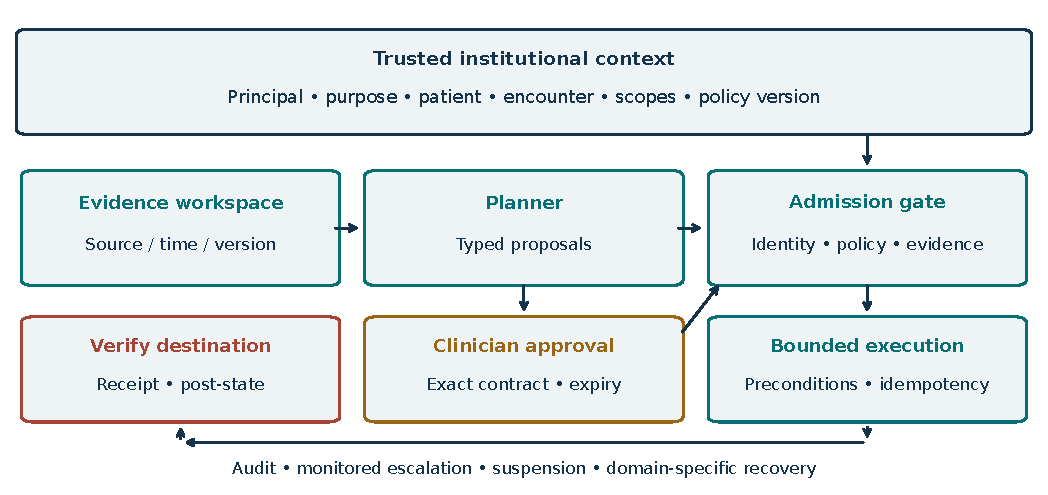
\includegraphics[width=\textwidth]{figures/fig3_caa_framework.pdf}
\caption{Proposed Clinical Action Assurance architecture. Trusted institutional identity and policy constrain the planner; exact-contract approval and current-state checks precede bounded execution. Destination verification and monitored escalation follow execution. The diagram is a proposed design, not a clinically validated system.}\label{fig:caa}
\end{figure*}

\subsection{Action contract and admission semantics}
A minimal action contract can be represented as
\begin{equation}
\kappa=(u,e,\mathrm{op},\mathbf{x},\mathbf{v},\mathcal{E},[t_0,t_1],\alpha,k),
\end{equation}
where $u$ and $e$ bind patient and encounter; $\mathrm{op}$ and $\mathbf{x}$ identify a typed operation and its arguments; $\mathbf{v}$ specifies required resource versions; $\mathcal{E}$ identifies supporting evidence; $[t_0,t_1]$ is the validity interval; $\alpha$ identifies approval; and $k$ is an idempotency key. The principal, purpose, and policy version must be bound in the contract or in trusted context used to validate it. Approval should refer to canonical contract content excluding the approval token itself, avoiding circular digest construction.

For policy $\theta$, let
\begin{equation}
G_\theta(\kappa)=I\wedge S\wedge V\wedge P\wedge E\wedge A\wedge L,
\end{equation}
where $I$ checks identity/encounter binding, $S$ allowed scope, $V$ current resource preconditions, $P$ domain constraints, $E$ evidence admissibility/freshness, $A$ approval, and $L$ temporal and operational limits. Each obligation should be true, false, or unresolved. A false obligation denies execution; an unresolved obligation defers it for resolution. Absence of a check is not permission. This conjunction is a control specification, not a probabilistic safety guarantee. In particular, domain-rule completeness and clinical evidence correctness are assumptions that need independent assessment.

\subsection{Approval and execution}
A clinician should review the actual proposed effect, its evidence, current patient context, and alternatives. Approval must be bound to the exact canonical payload, resource versions, and relevant policy. Mutation after approval invalidates that approval. A digest detects content change but does not authenticate the reviewer; production systems require genuine identity, authorization, secure token handling, and appropriate nonrepudiation controls.

The adapter should expose the minimum permitted operation set and reject requests that attempt to bypass preconditions. Execution should atomically enforce the destination state version wherever the underlying system allows it. A request key must map to one exact payload: repeated identical requests can return an established receipt, but changed content with the same key must fail. Revoked permissions or changed policy should remain effective even during retry handling. Technical success must be followed by checks of patient, operation, destination effect, and relevant state. A mismatch after commitment triggers reconciliation and escalation; it cannot retroactively make the effect disappear.

\subsection{Worked illustrative workflow}
Consider creation of a follow-up review task from a synthetic observation. The planner proposes a typed task for SYNTHETIC-P001 in SYNTHETIC-E001, referencing observation version 3. Trusted context permits only that task type and identifies an authorized reviewer. A clinician approval binds the proposal digest and expiry. If the observation changes to version 4 before commitment, the adapter rejects the stale precondition and requests a new review. If the write commits but its network response is lost, a retry with the same payload/key retrieves the established receipt. If the destination reports another patient or an unexpected task, the system escalates the unknown or mismatched effect.

The accompanying in-memory implementation illustrates these software obligations. It uses synthetic identifiers, a single task operation, explicit state versions, approval digests, an idempotency registry, and receipt checks. It has no LLM, live EHR, authenticated clinical identity, or clinically validated rule set. Its negative and retry tests are software invariant tests, not evidence that autonomous care is safe. This narrow example is intentionally reviewable: it demonstrates what must be specified before a richer agent architecture can be assessed.

\subsection{Monitoring and recovery ownership}
Monitoring must detect both unexpected writes and expected effects that never occur. Every deferred or escalated item needs a receiving role, acknowledgement, deadline, and overdue response. An institution should define suspension criteria, version-change review, and domain-specific recovery. Audit records should preserve source/evidence identifiers, policy and model versions, proposed and executed payloads, approval identity, receipts, and relevant post-state. Detailed reasoning traces may expose sensitive data or provide misleading rationales; operational audit should prioritize necessary observable evidence and apply governance to its retention.

\section{Evaluation and Translation Agenda}
\subsection{Choose the unit and denominator before scoring}
Evaluation should distinguish content correctness, valid tool invocation, correct destination action, completed workflow, and patient outcomes. A single task rate cannot summarize all five. Table~\ref{tab:metrics} proposes a denominator-aware vocabulary. Report omissions, abstentions, and excluded episodes; otherwise a system can appear safer merely by attempting fewer difficult cases.

For a diagnostic selective-prediction illustration with retention decision $q_i\in\{0,1\}$, define coverage and retained diagnostic error as
\begin{align}
C&=\frac{1}{n}\sum_{i=1}^{n}q_i,\\
R_{\mathrm{dx}}&=\frac{\sum_i q_i\,\mathbf{1}(\widehat{y}_i\ne y_i)}{\sum_i q_i}.
\end{align}
$R_{\mathrm{dx}}$ is undefined if no cases are retained. Such a conditional diagnostic measure differs from an action measure such as
\begin{equation}
R_{\mathrm{effect}}=\frac{N_{\mathrm{unsafe\ committed\ effects}}}{N_{\mathrm{committed\ effects\ assessed}}}.
\end{equation}
An episode-level analysis must additionally include inappropriate omissions, timing, and consequences. Low retained diagnostic error cannot be transferred to $R_{\mathrm{effect}}$ without directly evaluating the relevant actions. Calibration and selective prediction literature provide useful methods \cite{calibration2017,selective2017}; semantic uncertainty research supplies additional informational signals \cite{semanticentropy2024}. Their interpretation requires validation under the actual clinical workflow and distribution.

\begin{table}[t]\caption{Endpoint vocabulary and required denominators}\label{tab:metrics}\centering\footnotesize
\begin{tabularx}{\columnwidth}{@{}p{.35\columnwidth}Y@{}}\toprule
Endpoint & Required reporting unit \\ \midrule
Content correctness & Labeled answers/cases; label source.\\
Tool validity & Attempted calls; protocol and arguments.\\
Correct committed effect & Assessed destination effects; state predicate.\\
Workflow completion & Eligible episodes, full success criteria, timeout.\\
Selective coverage/risk & Eligible versus retained cases; exclusions.\\
Unsafe action/omission & Actions and eligible episodes; harm definition.\\
Human burden & Review time, interruptions, fallback load.\\
Patient/access outcome & Patients/episodes and follow-up; comparator.\\ \bottomrule
\end{tabularx}\end{table}

\subsection{Comparison and adjudication}
Comparators should include conventional automation, single-model assistance, and the existing human workflow when relevant. Budgets must be matched or explicitly analyzed: tool calls, tokens, time, retrieval access, feedback, and human oversight can determine an apparent architecture advantage. Model, prompt, memory, policy, tool, and evidence versions should be fixed and reported. Repeated stochastic runs are computational repeats, not additional independent patients.

Action adjudication needs blinded clinical expertise where appropriateness is material, execution-grounded checks where state changes matter, and a reproducible definition of harm and omission. Automated judges require validation against an appropriate human standard; overall agreement can conceal poor detection of rare serious errors. Report confidence intervals at the correct clustering level, distributions of failure severity, and incomplete/timeout trajectories. Subgroup analyses should evaluate both coverage and errors because selective routing can shift workload or access unequally.

\subsection{Staged clinical translation}
Figure~\ref{fig:translation} proposes six stages. Task specification defines eligible cases, allowable effects, human responsibilities, and failure recovery. Offline testing combines clinically meaningful tasks with adverse-state and security stress tests. Shadow evaluation measures performance under real workflow timing without committing effects. A clinician-approved pilot then assesses actual operational consequences with bounded permissions and monitored fallback. Prospective comparative evaluation examines patient, access, workload, and resource outcomes. Ongoing monitoring revalidates changes to models, memory, tools, data distributions, and institutional policies.

\begin{figure*}[t]\centering
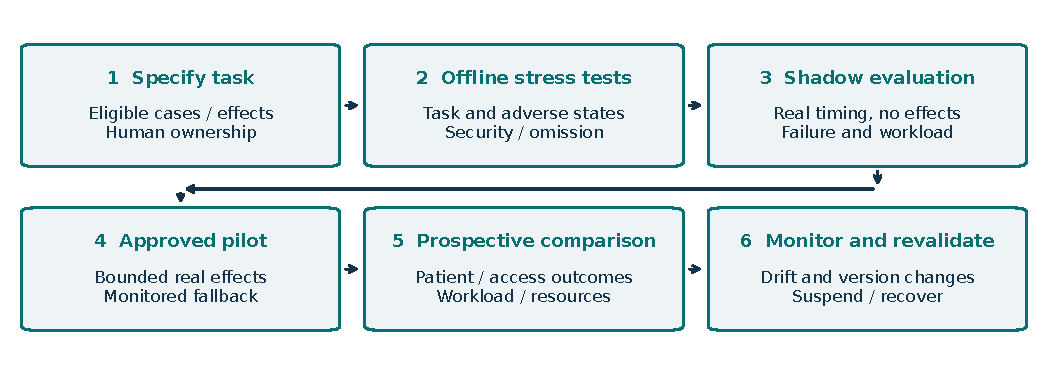
\includegraphics[width=\textwidth]{figures/fig5_translation.pdf}
\caption{Proposed staged translation, with evidence obligations at each stage. Progression is conditional on workflow-specific results and governance; these stages are not a regulatory certification pathway.}\label{fig:translation}
\end{figure*}

Reporting guidance should match the actual study. DECIDE-AI informs early clinical evaluation \cite{decideai2022}; SPIRIT-AI and CONSORT-AI support protocol and trial reporting \cite{spiritai2020,consortai2020}, alongside updated general trial guidance \cite{consort2025}. TRIPOD-LLM and STARD-AI address relevant prediction and diagnostic reporting \cite{tripodllm2025,stardai2025}. These guidelines improve transparent descriptions; they do not substitute for suitable design, clinical oversight, or evidence of benefit.

\section{Discussion and Research Priorities}
\subsection{What action assurance adds}
The selected literature demonstrates increasingly capable interaction with tools and complex environments. It also makes the gap between a local success and a completed episode visible. Action assurance offers a common language for that gap. By separating proposal, admissibility, execution, and effect verification, CAA makes obligations testable without asserting that one architecture is always preferred. A clinician can reject a contract, a destination can reject a stale version, and a receipt can reveal a mismatch independently of how persuasive the planner's explanation appears.

This approach connects rather than replaces clinical reasoning and governance. Technical scope controls can prevent prohibited operations while still allowing a clinically wrong permitted proposal. Clinical review can improve judgment while still missing a stale resource or duplicate write. Institutions need both suitable reasoning evidence and enforceable effect boundaries. Administrative tasks likewise warrant attention: incorrect documentation or payer submissions can delay care even without direct treatment decisions.

\subsection{Tradeoffs and implementation gaps}
Fine-grained approval and verification add latency and clinician work. If every action is deferred, apparent safety may reflect an unusable system. If review is compressed into a generic approval button, its protection may be illusory. Evaluation should therefore measure review quality, time, interrupted work, delayed care, and responsibility for unresolved episodes. Optimal boundaries may differ across reversible administrative tasks, medication-related actions, and longitudinal management.

Interoperability helps expose data and operations but does not eliminate heterogeneous semantics. A standard resource may represent a request, an accepted task, or a completed effect depending on destination behavior. Cross-system preconditions and idempotency may be unavailable. Likewise, authenticated identity is necessary but not sufficient when upstream patient matching or encounter context is wrong. CAA should be adapted to a documented threat model and workflow, with residual uncertainty acknowledged.

\subsection{Limitations of this review}
Purposive selection favors reports that illuminate observable agency and execution; it cannot estimate the proportion of systems that meet any assurance requirement. Only PubMed and arXiv support the reproducible discovery inventory, with targeted retrieval adding primary conference and journal material. Terminology and indexing may omit relevant systems, and inclusion of preprints makes some evidence provisional. Agent versions evolve rapidly, so reported rates apply to cited configurations and snapshots.

AI-assisted extraction can miss methodological details and cannot stand in for independent clinical verification. One selected source is abstract-only. The interrupted original workspace required a rebuild; the current audit distinguishes refreshed records from unavailable historical exports. We do not provide formal risk-of-bias assessment, pooled efficacy estimates, or new clinical experiments. CAA synthesizes existing ideas and may overlap with other governance frameworks; its novelty lies in the explicit action/effect/authority lens and reviewable operational contract, not a claim of first invention. Its synthetic implementation is deliberately incomplete for production.

\subsection{Outstanding questions}
\begin{enumerate}
\item Which decision-time signals predict unsafe action effects and clinically important omissions, rather than only diagnostic disagreement?
\item How can approvals remain valid across changing evidence and multiple clinical systems with limited transactional support?
\item What level of human review improves safety without unacceptable interruption, delay, or automation bias?
\item How should memory, model, retrieval, and policy changes trigger revalidation, including subgroup coverage and access?
\item Which prospective designs can identify benefit and harm attributable to a specific bounded authority, with adequate follow-up and accountable recovery?
\end{enumerate}

\section{Conclusion}
Healthcare agents should be evaluated according to what they observe, propose, commit, and verify, together with the authority that permits those effects. The selected evidence spans informational, interactive, artifact, and sandbox capabilities; it does not justify inferring live clinical benefit from aggregate benchmark success. Clinical Action Assurance provides a proposed structure for patient binding, evidence provenance, approval-bound contracts, current-state admission, bounded execution, and monitored effect verification. Its utility and clinical tradeoffs require further empirical assessment. Progress toward reliable clinical agency depends on connecting execution-level evidence with human workload, omissions, equitable access, and patient outcomes.

\section*{Data, Code, and AI Assistance}
Sources, evidence registers, original figures, build scripts, and a synthetic implementation are available in the accompanying repository at \url{https://github.com/ignitesoftlabs-pixel/research/tree/main/agentic-healthcare-review}. No patient-level data or publisher reading copies are redistributed. AI assisted discovery, extraction, synthesis, writing, and code generation. Independent human and clinical verification has not yet been documented; this version is a research draft. The implementation is illustrative software, with no clinical deployment or new patient experiment. Author identity, contributions, conflicts, funding, and required disclosures must be completed by the submitting authors.
\balance
\bibliographystyle{IEEEtran}
\bibliography{references}
\end{document}
